\chapter{Fundamentação teórica}

\section{Desenvolvimento de software} % (fold)
\label{sec:desenvolvimento_de_software}

% section desenvolvimento_de_software (end)

\subsection{Métodos tradicionais} % (fold)
\label{sub:metodos_tradicionais}

A base para diversos métodos de desenvolvimento que vêm sendo utilizado há décadas na indústria do software – por isso métodos tradicionais – é o modelo em cascata. Ele sugere uma abordagem sistemática e sequencial para o desenvolvimento de software que começa com a especificação dos requisitos pelo cliente e progire ao longo do planejamento, modelagem, construção, e implantação, culminando na manutenção progressiva do software acabado \cite{Pressman}.

\citeonline{XPTeles} e \citeonline{BDDRodrigo} fazem um apanhado sobre a relação entre o modelo cascata com os processos de produção industriais tayloristas. Estes processos tem como premissas o determinismo e a especialização. Dessa forma, isso leva ao desenvolvimento em cascata a especializar o desenvolvimento, ou seja, separar papéis na equipe de desenvolvimento onde cada um tem uma única responsabilidade. Além disso, existe uma busca pelo determinismo, que ganha força ao ser amparado pelo famosa curva de custos de correção do software por tempo transcorrido desde o início do processo \cite{Boehm}, mostrada na Figura \ref{img:custo-cascata}.

\begin{figure}[h]
  \center
  \caption{O custo das modificações no modelo tradicional - Fonte: \cite{XPKent}}
  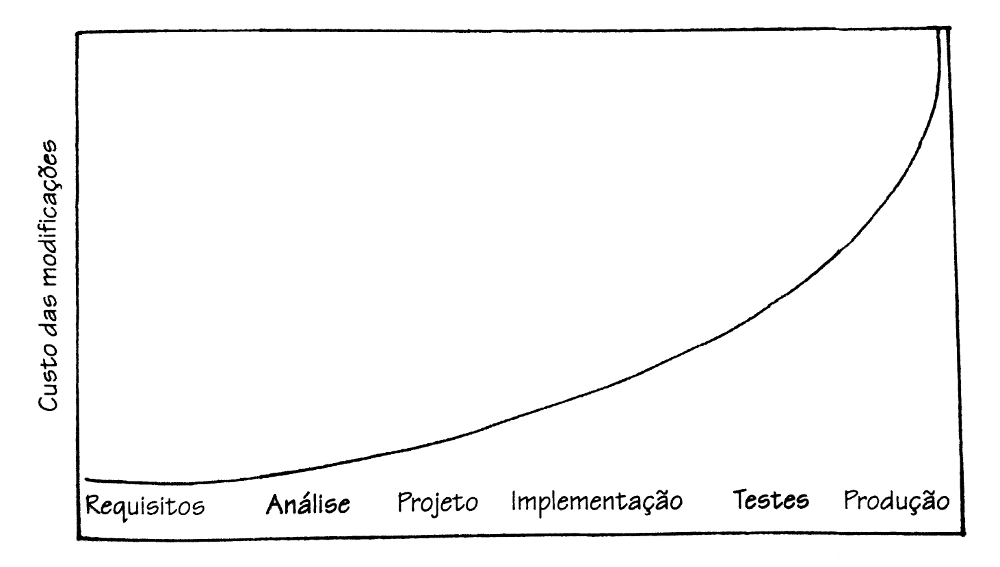
\includegraphics[scale=0.35]{images/custo-cascata}
  \label{img:custo-cascata}
\end{figure}

Esta busca pelo determinismo fez com que se pensasse, de forma completamente equivocada, que ao tentar com bastante afinco, consegue-se antecipar todo o conjunto de requisitos e reduzir os custos eliminando as mudanças \cite{TheBusinessOfInnovation}.

Ainda se baseando no processo de produção industrial, desta vez no gerenciamento fordista, outra premissa extremamente equivocada englobada pelo modelo cascada é a de que desenvolvimento de software é um trabalho executado por trabalhadores manuais e não um trabalhadores do conhecimento \cite[38]{XPTeles}.

Embora o desenvolvimento em cascata seja reconhecidamente ineficaz, ainda é o processo mais utilizado para o desenvolvimento de sistemas \cite{XPTeles}.

% subsection metodos_tradicionais (end)


\subsection{Agilismo} % (fold)
\label{sub:agilismo}

TODO: Rodrigo: [Esta seção pode ser bem expandida (aqui pode ser melhor explicado o lance dos ``equívocos"\ da engenharia de software tradicional). Fale da diferença conceitual entre agilismo e tradicionalismo; explique as curvas de Boehm (Software Engineering Economics, 1981) e de Beck (Extreme Programming Explained, 1999); cite (sem maiores aprofundamentos) a origem do agilismo no Toyota Way; explique iteração e release no contexto de um processo ágil.]

Em 2001 um grupo de dezessete especialistas, reconhecidos pela comunidade como grandes nomes do desenvolvimento software, se reuniram para discutir sobre um crescente conjunto de métodos que vinham surgindo e decidiram usar o termo Agilismo para descrever essa nova geração de métodos ágeis \cite{AgileStory}. Na mesma reunião, eles também escreveram o Manifesto Ágil \cite{AgileManifesto}, delineando um conjunto de valores e princípios que, em resumo, trilham um caminho para a eliminação de documentação e processos desnecessários, buscando a simplicidade, com foco na geração de valor e proximidade com o cliente, além de possibilitar respostas rápidas e eficazes às mudanças.

\begin{figure}[h]
  \center
  \caption{O custo das modificações no modelo ágil - Fonte: \cite{XPKent}}
  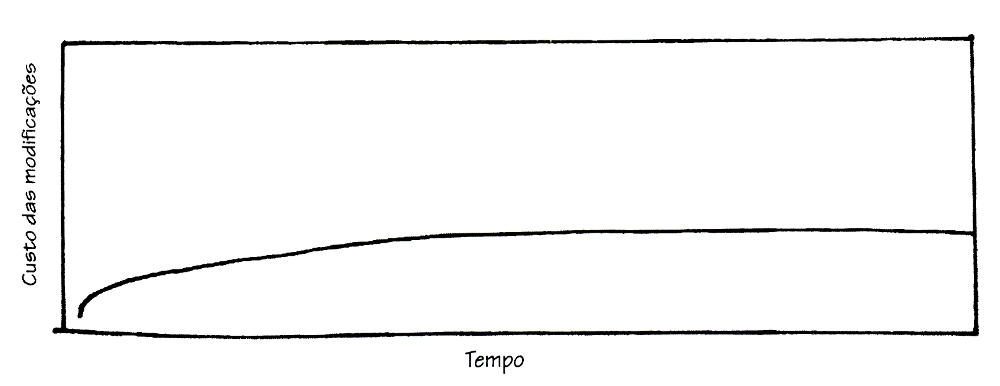
\includegraphics[scale=0.45]{images/custo-agile}
  \label{img:custo-agile}
\end{figure}

Pode-se dizer então, que o Desenvolvendo Ágil, ou Agilismo, é um rótulo genérico para os métodos de desenvolvimento de software baseados no Manifesto Ágil \cite{BDDRodrigo}.

% subsection agilismo (end)

% section desenvolvimento_de_software (end)

\section{Tipos de teste}
\label{sec:tipos_de_teste}

TODO: Rodrigo: [Explique melhor (e com exemplos) cada tipo de teste, relacionando as definiçoes na literatura ágil com as definições na literatura tradicional.]

\subsection{Testes de unidade}
\label{sub:testes_de_unidade}

Testes de unidade são testes nos quais unidades individuais do sistema são testadas para determinar se estão aptas para uso. Uma unidade é a menor parte testável de uma aplicação. Em programação procedural uma unidade pode ser uma função ou \textit{procedure}. Já em programação orientada a objetos, uma unidade pode ser um método.

% subsection testes_de_unidade (end)

\subsection{Testes de integração}
\label{sub:testes_de_integracao}

Teste de integração testam as integrações do código com o mundo exterior. Podem ser um teste que se comunique através da rede, tenha contato com o sistema de arquivos ou deixe os limites de seu próprio processo \cite{ArtOfAgileDevelopment}.

% subsection testes_de_integracao (end)

\subsection{Testes de aceitação}
\label{sub:testes_de_aceitacao}

Testes de aceitação são especificações para o comportamento e funcionalidade de um sistema. Os testes de aceitação nos mostram se o sistema se comporta corretamente pela perspectiva de um usuário, sem nos dizer nada sobre como o sistema implementa esse comportamento \cite{TestDrivenKoskela}.

% subsection testes_de_aceitacao (end)

% section tipos_de_teste (end)